\documentclass[sigconf]{acmart}
\usepackage{booktabs}
\usepackage{placeins}
\usepackage{algorithmicx}
\usepackage[noend]{algpseudocode}
\usepackage{algorithm}
\usepackage{subcaption}


%% \BibTeX command to typeset BibTeX logo in the docs
\AtBeginDocument{%
  \providecommand\BibTeX{{%
    \normalfont B\kern-0.5em{\scshape i\kern-0.25em b}\kern-0.8em\TeX}}}

%% These commands are for a PROCEEDINGS abstract or paper.
\settopmatter{printacmref=false} % Removes citation information below abstract
\renewcommand\footnotetextcopyrightpermission[1]{} % removes footnote with conference information in 

\acmConference[AGML LAB]{Statistical Learning Theory LAB}{August 9}{Jena, Germany}


\graphicspath{{graphics/}}

\definecolor{myblue}{RGB}{46, 59, 160}
\hypersetup{
    pdfstartpage=1,
    pdfstartview = FitB,
    pdfpagelayout=SinglePage,
    pdftitle={Project Report},
    pdfsubject={Statistical Learning Theory},
    pdfauthor={Maurice Wenig},
    pdfcreator={Maurice Wenig},
    pdfproducer={Maurice Wenig},
    pdfkeywords={meta, information, pdf, hyperref, latex},
    colorlinks=true,
    linkcolor=myblue,
    citecolor=myblue
}

%----- new commands
\newcommand{\Romannumeral}[1]{\MakeUppercase{\romannumeral #1}}
\newcommand{\set}[1]{\{#1\}}
\newcommand{\abs}[1]{\left\vert #1 \right\vert}
\newcommand{\norm}[1]{\left\| #1 \right\|}
\newcommand{\skal}[2]{\left\langle #1 | #2 \right\rangle}
\newcommand{\script}[1]{
    skripte/aufgabe#1.py
    \lstinputlisting{skripte/aufgabe#1.py}
}
%----- defs
\def\notiff{\mathrel{{\ooalign{\hidewidth$\not\phantom{"}$\hidewidth\cr$\iff$}}}}
\def\R{\mathbb{R}}
\def\bbone{\text{\usefont{U}{bbold}{m}{n}1}}
\def\1{\mathbb{1}}
\def\T{\top}
\def\ndy{
    \textcolor{red} {\hfill not done yet!}
    \reversemarginpar
    \marginpar{\raggedleft\textcolor{red}{\rule{2mm}{2mm}}}
}
\def\ghostline{\hfill\vspace*{-5mm}}

\begin{document}

%%
%% The "title" command has an optional parameter,
%% allowing the author to define a "short title" to be used in page headers.
% Fast Entity Resolution With Mock Labels and Sorted Integer Sets
\title[Project Report]{Project Report\\\large Statistical Learning Theory LAB}

%%
%% The "author" command and its associated commands are used to define
%% the authors and their affiliations.

\author{Maurice Wenig}
\affiliation{%
	\institution{Friedrich Schiller University Jena}
	\country{Germany}}
\email{maurice.wenig@uni-jena.de}


%%
%% This command processes the author and affiliation and title
%% information and builds the first part of the formatted document.
\maketitle

% \let\thefootnote\relax\footnotetext{AEPRO 2022, March 1, Jena, Germany. Copyright \copyright 2022 for this paper by its authors. Use permitted under Creative Commons License Attribution 4.0 International (CC BY 4.0).}


\section{Introduction}
The context of this project are rating systems.
Users can rate specific items with a score from 0 to 4.
The goal is then, to predict the rating of an item for a specific user.
To achieve this, we are given training data, that specifies how users rated specific items.
This data can be turned into the rating matrix \cite[Chapter~1, Section~3]{Aggarwal2016}, where the items form the columns, and the users form the rows.
This rating matrix is naturally sparse, as can be seen in \autoref{fig:intro:rating_matrix}, where white pixels are missing data points.
\begin{figure}[!htb]
	\centering
	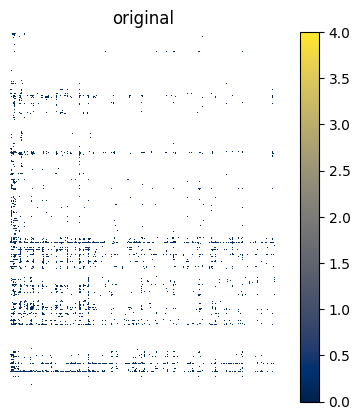
\includegraphics[scale=0.6]{matrix_original.png}
	\caption{Sparse rating matrix}
	\label{fig:intro:rating_matrix}
\end{figure}

The user and item ratings also have a long tail, meaning that there are only a few users who rated a lot of items, and a lot of users, who rated very few items.
The long tail effect for items is not as strong as it is for users in the training data.
This can be observed in \autoref{fig:into:long_tail}, where users and items have been sorted by number of ratings.
\begin{figure}[!htb]
	\begin{subfigure}{0.2\textwidth}
		\centering
		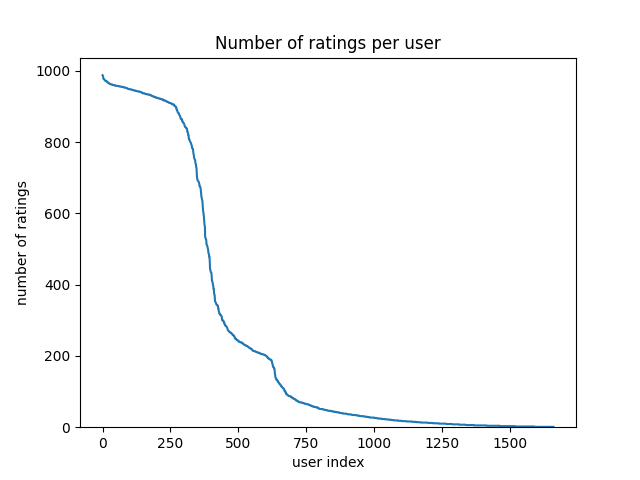
\includegraphics[scale=0.23]{user_frequency.png}
	\end{subfigure}
	\begin{subfigure}{0.2\textwidth}
		\centering
		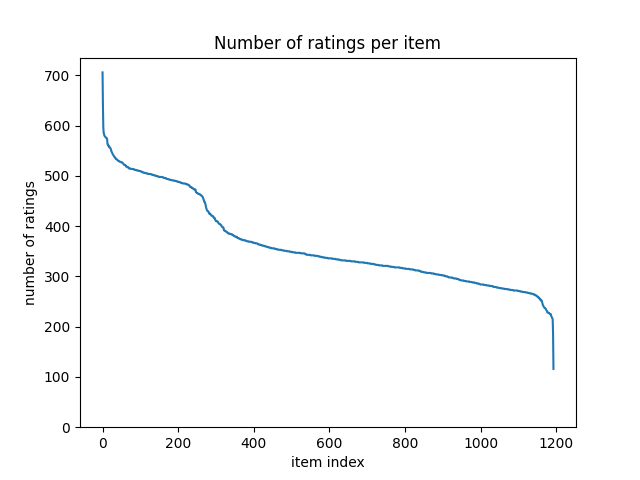
\includegraphics[scale=0.23]{item_frequency.png}
	\end{subfigure}
	\caption{Long tail of user and item ratings}
	\label{fig:into:long_tail}
\end{figure}
\FloatBarrier


\section{Methods}
\subsection{Neighbourhood-Based Methods}
\label{sec:methods:neighbourhood}

\subsubsection{User-Based Recommender}
\label{sec:methods:neighbourhood:user}
The user-based recommender compares users based on their rated items. An item rating from a user is then predicted based on ratings of that item from similar users.
The similarity measure used to compare users is Pearson:
$$\text{Sim}(u, v) = \frac{\sum\limits_{i\in I_{uv}} w_i \cdot s_{ui} s_{vi}}{\sqrt{\sum\limits_{i\in I_{uv}} w_i \cdot  s_{ui}} \cdot \sqrt{\sum\limits_{i\in I_{uv}} w_i \cdot  z_{vi}}}$$
where $I_{uv}$ are the items that both users $u$ and $v$ have rated, $s_{ui} = r_{ui} - \mu_u$ is the centered rating from user $u$.
The mean rating $\mu_u$ can be calculated individually for every comparison, based on only the common items, or it can be calculated once for every user, based on all their rated items.
$w_i = \log\frac{\text{\# users}}{\text{\# users who rated } i}$ are item weights to combat the impact of the long tail in the number of item ratings.

To prefer users with more common items, the similarites of users with less than $\beta$ common items are made smaller.
$$\text{Sim}(u, v) \gets \text{Sim}(u, v) \cdot \frac{\min\set{\abs{I_{uv}}, \beta}}{\beta}$$

The hyper parameter $\alpha$ can be used to amplify the importance of similarity.
$$\text{Sim}(u, v) \gets \text{Sim}(u, v)^\alpha$$

Based on these similarities, a peer group $P_u(i)$ of users is determined. For this, the users are sorted by similarity.
To improve efficiency in the online phase, the sorting is done in the offline phase.
For this, the similarities between every user $u, v$ are saved in the similarity matrix.
The order of peers for a specific user is then determined by sorting the respective row vector.

In the online phase, this order is simply applied. Users are then removed, if they have not rated them item $i$, or their similarity to user $u$ is below a certain threshold $S_{min}$.
The top $k$ remaining users are then the peer group $P_u(i)$.

The predicted item rating from a user is then calculated as a sum of ratings from similar users, weighted with their relative similarity.
The means and variances of the user ratings are normalized to not influence the prediction.
$$\hat{r}_{ui} = \mu_u + \sigma_u \cdot \frac{\sum\limits_{v \in P_u(i)} \text{Sim}(u, v) \cdot z_{vi}}{\sum\limits_{v \in P_u(i)} \abs{\text{Sim}(u, v)}}$$
where $z_{ui} = s_{ui} / \sigma_u$ is the normalized rating, $\sigma_u$ the variance of the ratings of user $u$.
All of this and the reasoning behind it is described in \cite[Chapter~2, Section~3.1]{Aggarwal2016}.

If the user has only ever given one distinct rating, the variance is set to an arbitrary value of 1.

\hypertarget{special_cases}{}
In special cases where the user or the item has never been seen before, similarities can not be calculated. In those special cases, the ratings were predicted in a different way:
\begin{itemize}
	\item user and item unknown: predict average between minimum and maximum possible rating
	\item user unknown, item known: predict average rating of that item
	\item user known, item unknown: predict average rating of that user
\end{itemize}
Also, if the original item rating of the user is known, this original rating can be predicted.

The best performing hyper parameters were the following:
\begin{itemize}
	\item $k = 50$ neighbours in peer group
	\item $\alpha = 1$, not amplifying importance of similarity
	\item $S_{min} = 0.4$ minimum similarity
	\item $\beta = 4$ common dimensions before similarity reduction
\end{itemize}


\subsubsection{Item-Based Recommender}
\label{sec:methods:neighbourhood:item}
The item-based recommender compares items based on their user ratings. An item rating from a user is then predicted based on ratings of similar items from that user.
It functions very similar to the user-based recommender. The similarity function is adapted to still use user means $\mu_u$ instead of item means $\mu_i$ to normalize user preferences.
The predicted rating is then a weighted sum of similar items, the user has rated \cite[Chapter~2, Section~3.2]{Aggarwal2016}.
$$\hat{r}_{ui} = \frac{\sum\limits_{j \in P_i(u)} \text{Sim}(i, j) \cdot r_{uj}}{\sum\limits_{j \in P_i(u)} \abs{\text{Sim}(i, j)}}$$

The best performing hyper parameters were the following:
\begin{itemize}
	\item $k = 50$ neighbours in peer group
	\item $\alpha = 1$, not amplifying importance of similarity
	\item $S_{min} = 0.6$ minimum similarity
	\item $\beta = 6$ common dimensions before similarity reduction
\end{itemize}


\subsubsection{Clustering}
\label{sec:methods:neighbourhood:clustering}
To increase efficiency, the users/items can be clustered before the creation of the similarity matrix. This way, only users/items that are in the same cluster have to be compared.

This is done using an adapted version of K-means \cite[Chapter~2, Section~4]{Aggarwal2016}.
To account for the sparsity of the rankings matrix, the entries of the mean of a cluster are calculated using only vectors, where the entries are not missing in the respective dimensions.
The distance measure is also adapted. The distance between two vectors is calculated only with the common dimensions, where ratings are not missing.
The result is then divided by the number of common dimensions to get a distance measure that is independent of the number of common dimensions.

The number of clusters was tuned to get the best trade-off of performance and prediction quality.
This resulted in clustering with $K = 8$ for the user-based recommender.
Such a good trade-off could not be found for the item-based recommender.


\subsection[Factorization]{Factorization-Based Recommender}
\label{sec:methods:factorization}
In the factorization-based recommender, the users and items are assumed to be in a common latent factor space $R^f$ of user preferences $q_i$ and item characteristics $p_u$.
The rating $r_{ui}$ is then modelled as the user's interest in the item's characteristics. User and item biases are also taken into account.
$$\hat{r}_{ui} = q_i^\T p_u + \mu + b_i + b'_u$$

The goal is then to learn the factors $q_i, p_u$, such that the squared error function on the ratings of the training set is minimal.
$$\min\limits_{p, q, b} \sum\limits_{(u, i) \in \kappa} (r_{ui} - \hat{r}_{ui})^2 + \lambda \left(\norm{q_i}^2 + \norm{p_u}^2 + b_i^2 + {b'_u}^2\right)$$
with $\kappa$ as the set of $(u, i)$ pairs in the training set, $\lambda$ as the regularization parameter.
This model, its loss function, and ideas for solving this minimization problem are described in \cite{Koren2009}.

To achieve this minimzation, alternating least squares is used.
$q, p$ are initiated randomly.
Then, in each step, one of them is fixed and the other one is solved optimally.
This is done until the change of the vectors in $q, p$ is below a threshold $\epsilon$ or a maximum number of iterations is reached.

To optimally solve the minimization at each step, ridge regression is used \cite{Hoerl1970}.
Because they are independent, each of the summands are optimized individually.
\begin{gather*}
	\min\limits_{p_u, b'_u} \sum\limits_{i \in \kappa_u} \left((r_{ui} - b_i - \mu) - (q_i^\T p_u + b'_u)\right)^2 + \lambda \left(\norm{p_u}^2 + {b'_u}^2\right)\\
	\min\limits_{q_i, b_i} \sum\limits_{u \in \kappa_i} \left((r_{ui} - b'_u - \mu) - (q_i^\T p_u + b_i)\right)^2 + \lambda \left(\norm{q_i}^2 + b_i^2\right)
\end{gather*}
with $\kappa_u$ as the set of items that have been rated by $u$, $\kappa_i$ as the set of user that have rated $i$.

The ridge regression the boils down to solving the regularized normal equations:
\begin{gather*}
	\left(Q_{\kappa_u} {Q_{\kappa_u}}^\T + \lambda\bbone\right) p_u = Q_{\kappa_u} y_{\kappa_u}\\
	\left(P_{\kappa_i} {P_{\kappa_i}}^\T + \lambda\bbone\right) q_i = P_{\kappa_i} y_{\kappa_i}
\end{gather*}
with
\begin{align*}
	Q_{\kappa_u}  & = (q_{i_1}, \dots, q_{i_n})                                  \\
	y_{\kappa_u}  & = \vec{r}_{\kappa_u} - \vec{b}                               \\
	              & = (r_{ui_1}, \dots, r_{ui_n})^\T - (b_{i_1}, \dots, b_{i_n}) \\
	i, \dots, i_n & \in \kappa_u
\end{align*}
for determining $p_u$ and
\begin{align*}
	P_{\kappa_i}    & = (p_{u_1}, \dots, p_{u_n})                                      \\
	y_{\kappa_i}    & = \vec{r}_{\kappa_i} - \vec{b'}                                  \\
	                & = (r_{u_1 i}, \dots, r_{u_n i})^\T - (b'_{u_1}, \dots, b'_{u_n}) \\
	u_1, \dots, u_n & \in \kappa_i
\end{align*}
for determining $q_i$.

The biases can either be fixed or part of the optimization.
If the biases are fixed, $\mu$ is the overall mean rating in the training set, $b'_u = \mu_u - \mu$ is the mean user rating centered around the overall mean rating, $b_i = \mu_i - \mu$ is the mean item rating centered around the overall mean rating.
If the biases are part of the optimization, they are the affine part of the ridge regression at each step.
This affine part can be obtained by appending a constant 1 to the training vectors and reading its respective coefficient.

The special cases are handled in the same way as they are in the \hyperlink{special_cases}{User Based Recommender}.

The best performing hyper parameters were the following:
\begin{itemize}
	\item $\lambda = 5$ regularization parameter
	\item $f = 20$ latent dimensions
	\item biases not fixed
	\item $\epsilon = 10^{-2}$, max 20 iterations
\end{itemize}


\subsection[Hybrid]{Hybrid Recommender}
\label{sec:methods:hybrid}
The hybrid combines an array of $K$ recommenders. The predictions are a linear combination of the predictions of those recommenders.
$$\hat{r}_{ui} = \sum\limits_{k = 1}^{K} \alpha_k \hat{r}^{(k)}_{ui} = \vec{\alpha}^\T \vec{r}_{ui}$$

To learn $\vec{\alpha}$, the training set is separated into two parts: a fitting set, and a held out set.
The recommenders are then trained on the fitting set.
Then, the recommenders predict the labels of the held out set.
The optimal alpha can either minimize the mean absolute error
$$\mathcal{E}_1 = \frac{1}{m}\norm{R - \vec{R} \vec{\alpha}}_1$$
or the (half) mean squared error (MSE)
$$\mathcal{E}_2 = \frac{1}{2m}\norm{R - \vec{R} \vec{\alpha}}^2_2$$
$m$ as the number of samples in the held out set,
$R = (r_1, \dots, r_m)^\T$ as the vector of true ratings of the held out samples,
$\vec{R} = (\vec{r}_1, \dots, \vec{r}_m)^\T$ as the matrix of predictions on the held out samples.

$\vec{\alpha}$ is then optimized with gradient descent. Every entry is intialized with $\frac{1}{K}$.
At each step, $\vec{\alpha} \gets \vec{\alpha} - \gamma \nabla\mathcal{E}(\vec{\alpha})$ is pushed into the direction of the negative gradient of the error, scaled with a learning rate $\gamma$.
This is done until the error changes less than a threshold $\epsilon$, or the maxmimum amount of iterations is reached.
\begin{align*}
	\nabla\mathcal{E}_1(\vec{\alpha}) & = \frac{1}{m} \text{sign}\left(R - \vec{R} \vec{\alpha}\right)^\T \vec{R} \\
	\nabla\mathcal{E}_2(\vec{\alpha}) & = \frac{1}{m} \left(R - \vec{R} \vec{\alpha}\right)^\T \vec{R}
\end{align*}
This model, its error functions, and the gradient descent method are described in \cite[Chapter~6, Section~3]{Aggarwal2016}.

After $\vec{\alpha}$ has been determined, the predictors are trained on the whole training set to not miss out on information.
Special cases do not need to be handled, as they are handled in the individual recommenders.

The best performing hyper parameters were the following:
\begin{itemize}
	\item hybrid of clustered user-based recommender, unclustered item-based recommender, and factorization-based recommender
	\item optimize for MSE
	\item $\gamma = 1$ learning rate
	\item $\epsilon = 10^{-4}$, max 100 iterations
\end{itemize}

\begin{figure}[!htb]
	\centering
	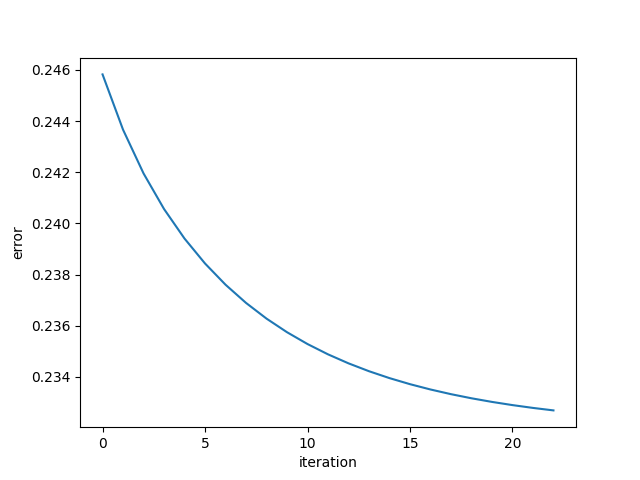
\includegraphics[scale=0.4]{descent.png}
	\caption{Hybrid error during gradient descent}\label{fig:hybrid_descent}
\end{figure}
It is worthy to note that the hybrid didn't improve much compared to the initial equal weights.
In \autoref{fig:hybrid_descent} you can see mean absolute error (MAE) of the hybrid recommender during the gradient descent of $\vec{\alpha}$.


\section{Results}
\subsection{Performance}
\label{sec:results:performance}
For time measurement, the recommenders were trained on \href{run:../input/train.csv}{\texttt{train.csv}} (435K samples) and evaluated on \href{run:../input/qualifying_blanc.csv}{\texttt{qualifying\_blanc.csv}} (109K samples).
\begin{table}[htbp]
	\caption{Run Time Comparison}
	\label{tab:results:run_time}
	\begin{tabular}{lrrr}
		\toprule
		Recommender   & offline phase & online phase \\
		\midrule
		user based    & 15.97s        & 6.84s        \\
		item based    & 44.3s         & 4.79s        \\
		factorization & 85.65s        & 0.53s        \\
		hybrid        & 304.1s        & 26.79s       \\
		\bottomrule
	\end{tabular}
\end{table}


\subsection{Error Scores}
\label{sec:results:errors}
The error scores were measured with cross validation on the training set, with $R = 8$ rotations.
Root mean squared error (RMSE) and MAE were calculated.
\begin{table}[htbp]
	\caption{Error Score Comparison}
	\label{tab:results:errors}
	\begin{tabular}{lrrr}
		\toprule
		Recommender   & RMSE  & MAE   \\
		\midrule
		user based    & 0.670 & 0.301 \\
		item based    & 0.569 & 0.222 \\
		factorization & 0.512 & 0.207 \\
		hybrid        & 0.496 & 0.193 \\
		\bottomrule
	\end{tabular}
\end{table}
\FloatBarrier


\subsection{Full Rating Ratrices}
\label{sec:results:full_matrix}
The recommenders can be used to fill the rest of the rating matrix with predictions. The resulting structures are visualized in \autoref{fig:results:full_matrices}.
\begin{figure}[!htb]
	\begin{subfigure}{0.2\textwidth}
		\centering
		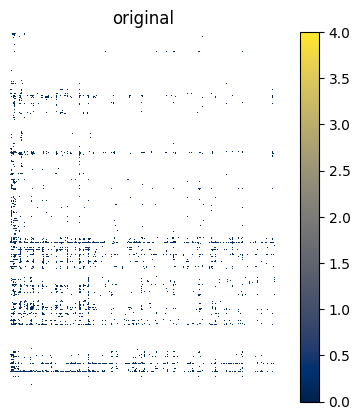
\includegraphics[scale=0.4]{matrix_original.png}
	\end{subfigure}
	\hfill\\
	\begin{subfigure}{0.2\textwidth}
		\centering
		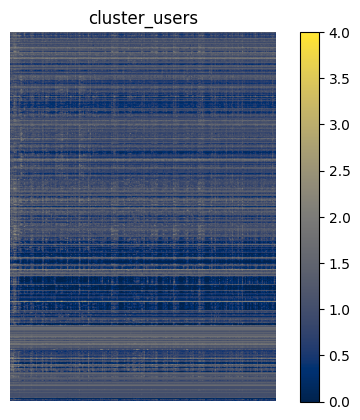
\includegraphics[scale=0.4]{matrix_cluster_users.png}
	\end{subfigure}
	\begin{subfigure}{0.2\textwidth}
		\centering
		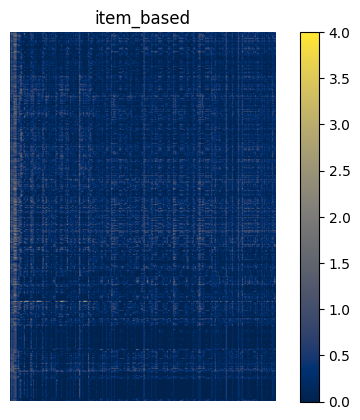
\includegraphics[scale=0.4]{matrix_item_based.png}
	\end{subfigure}
	\hfill
	\begin{subfigure}{0.2\textwidth}
		\centering
		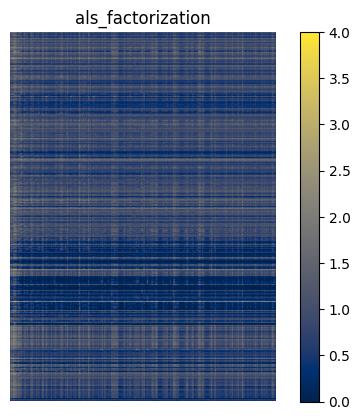
\includegraphics[scale=0.4]{matrix_als_factorization.png}
	\end{subfigure}
	\begin{subfigure}{0.2\textwidth}
		\centering
		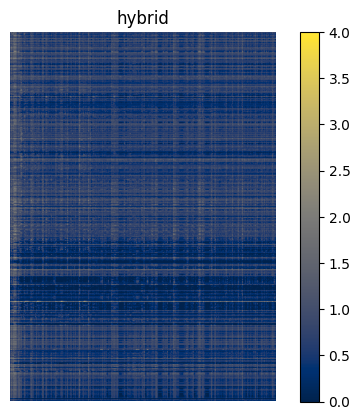
\includegraphics[scale=0.4]{matrix_hybrid.png}
	\end{subfigure}
	\caption{Rating matrix filled by recommenders}
	\label{fig:results:full_matrices}
\end{figure}
\FloatBarrier


\section{Conclusion}
I successfully implemented recommender systems, that predict item ratings for specific users.
My recommenders are slow, but the predictions are of high quality.
This can be seen on the \href{http://csujena.pythonanywhere.com/}{validation set}, where my hybrid recommender is the best scoring recommender at the time of writing, with a score of 0.530.

\typeout{}
\bibliographystyle{ACM-Reference-Format}
\bibliography{literature}


\end{document}
\endinput
%%
%% End of file `sample-sigconf.tex'.
